%%%%%%%%%%%%%%%%%%%%%%%%%%%%%%%%%%%%%%%%%%%%%%%%%%%%%%%%%%%%%%%%%%%%%%%%%%%%%%%%
%% Overall Approach
%%%%%%%%%%%%%%%%%%%%%%%%%%%%%%%%%%%%%%%%%%%%%%%%%%%%%%%%%%%%%%%%%%%%%%%%%%%%%%%%


\section{Overall modeling approach} \label{sec:modelapproach}

	We hypothesize that permanent set and structural damage are two separate and largely sequential mechanisms that underlie the mechanical response of BHVs. Thus, the life span of BHVs can by separated into three stages: early (up to 2-5 years),  intermediate (up to 10 years), and late stage (up to failure) (Fig. \ref{fig:hypothesis}). In the early stage, permanent set induces significant changes in BHV geometry while structural damage does not play a detectable role. This leads to increased stress and structural damage in the intermediate term which leads to failure in the late term. Thus, by compensating for the effect of permanent set on the geometry, we hypothesize that we can extend the life span of BHVs. We focus our model on the early stage of cyclic loading and build a solid foundation for modeling and simulating the later stages.


\begin{figure}[hbt]
\centering
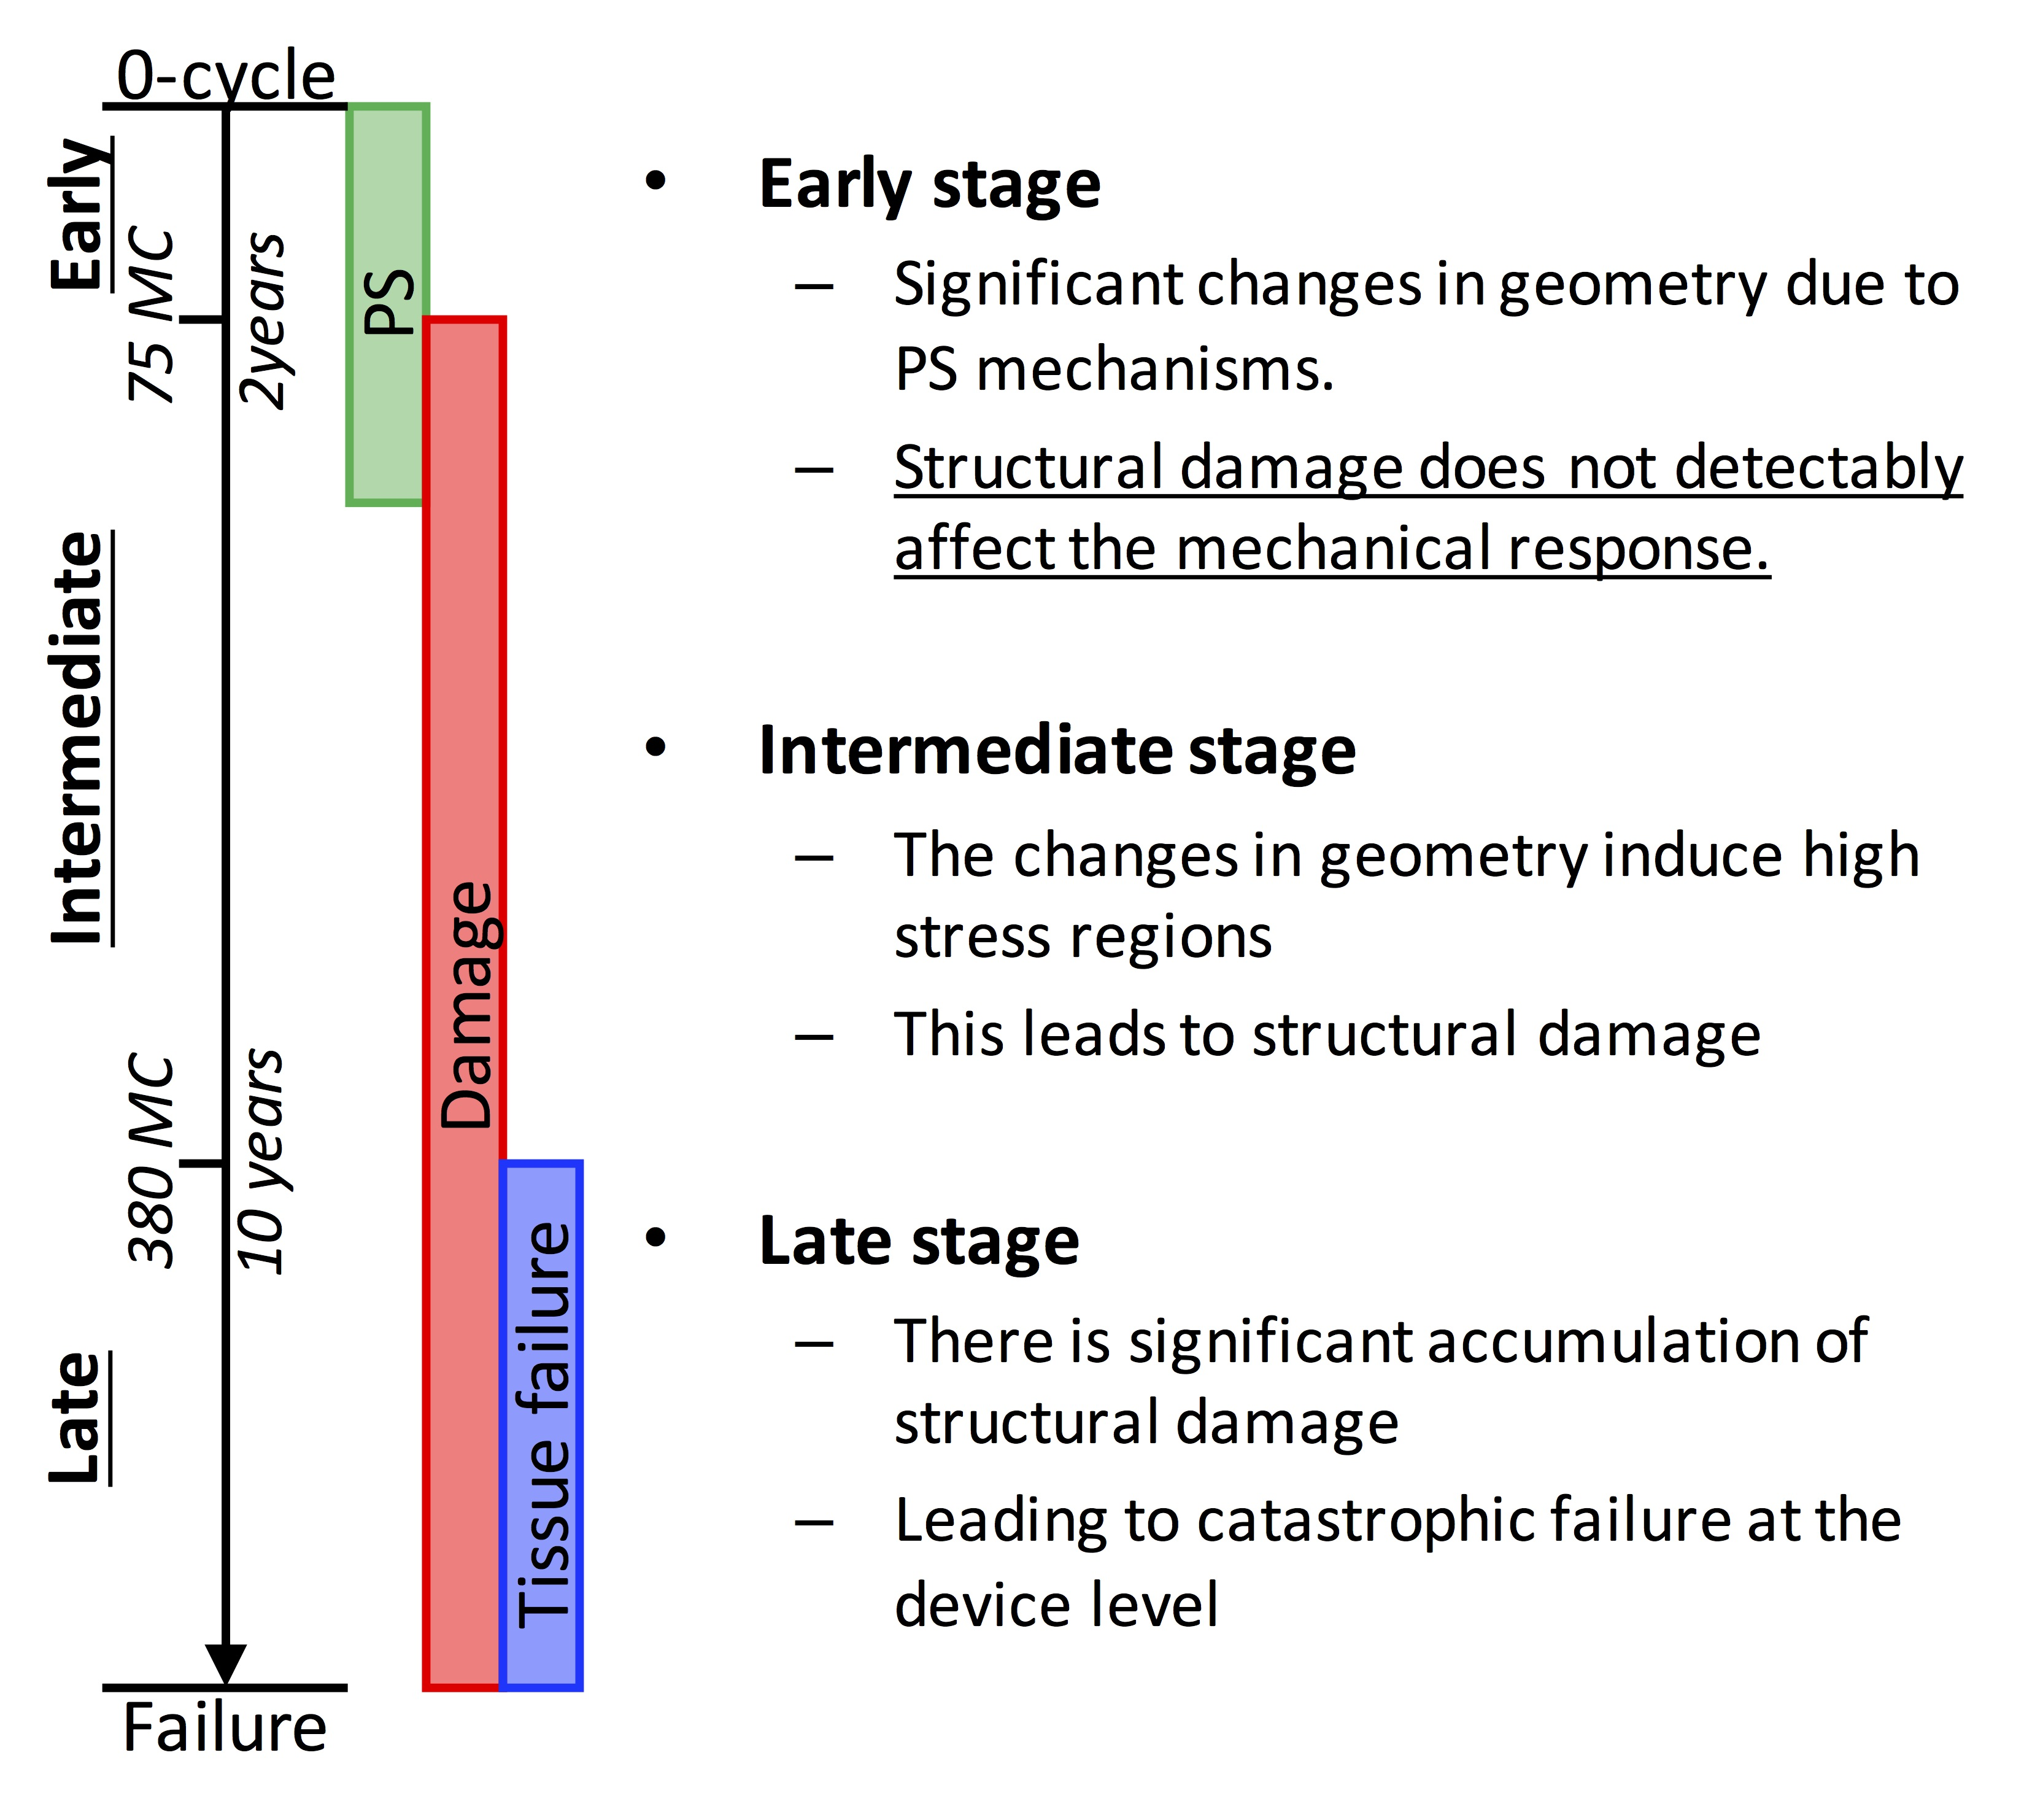
\includegraphics[width=4in]{Images/chapter4/figure2}
\caption{We speculate that the progression of structural damage and permanent set of BHV leaflets progress during long term cyclic loading can be separated into three stages: early, intermediate, and late.}
\label{fig:hypothesis}
\end{figure}


	We assume that permanent set is driven by the scission-healing behaviors of the GLUT polymer network in the non-fibrous EXL matrix, allowing for fractions of it to change in reference state (Fig. \ref{fig:PS}A). The formation of aldehyde bonds during crosslinking, as well as the occasional hydrolysis of the aldehyde bonds follows \emph{first order molecular kinetics} \cite{migneault_glutaraldehyde_2004}. Since this process drives the scission-healing of GLUT polymers and thus permanent set, we hypothesize that permanent set also follows first order kinetics. In addition, we note that the length scale of crosslinks formed by GLUT polymers ($\mathrm{nm}$) in the EXL matrix is several orders of magnitude smaller than that of the collagen fibers ($\mu \mathrm{m}$). Thus, we assume that the collagen fiber architecture does \emph{not} undergo scission-healing like the EXL matrix. Instead, the collagen fibers remain intact during cyclic loading. Rather, the collagen fiber architecture is convected by the changes in geometry that occurs with permanent set in the EXL matrix (Fig. \ref{fig:PS}B). \emph{We refer to this mechanism as structural convection, which is defined as applying a permanent deformation (elongation and rotation of collagen fibers, Fig. \ref{fig:structuralconvection}) to the collagen fiber architecture based on the change in the reference configuration}. Previously, we have shown that dense collagenous tissues deform under affine kinematics \cite{lee_presence_2015}. Since deformations during cyclic loading are in the elastic regime and cyclic loading (second) is on a time scale much shorter than that of permanent set (weeks), the only change in collagen fiber architecture on a cycle to cycle period is also under affine kinematics. Therefore, we also assume that the convection of collagen fiber architecture due to permanent set is under affine kinematics as well. Thus, our approach is based on using the permanent set effect to model the evolving properties of the EXL matrix, determine the change in reference configuration and convect collagen fiber architecture, which then allows us to determine the change in mechanical response of the collagen fibers using structural models. 


\begin{figure}[hbt]
\centering
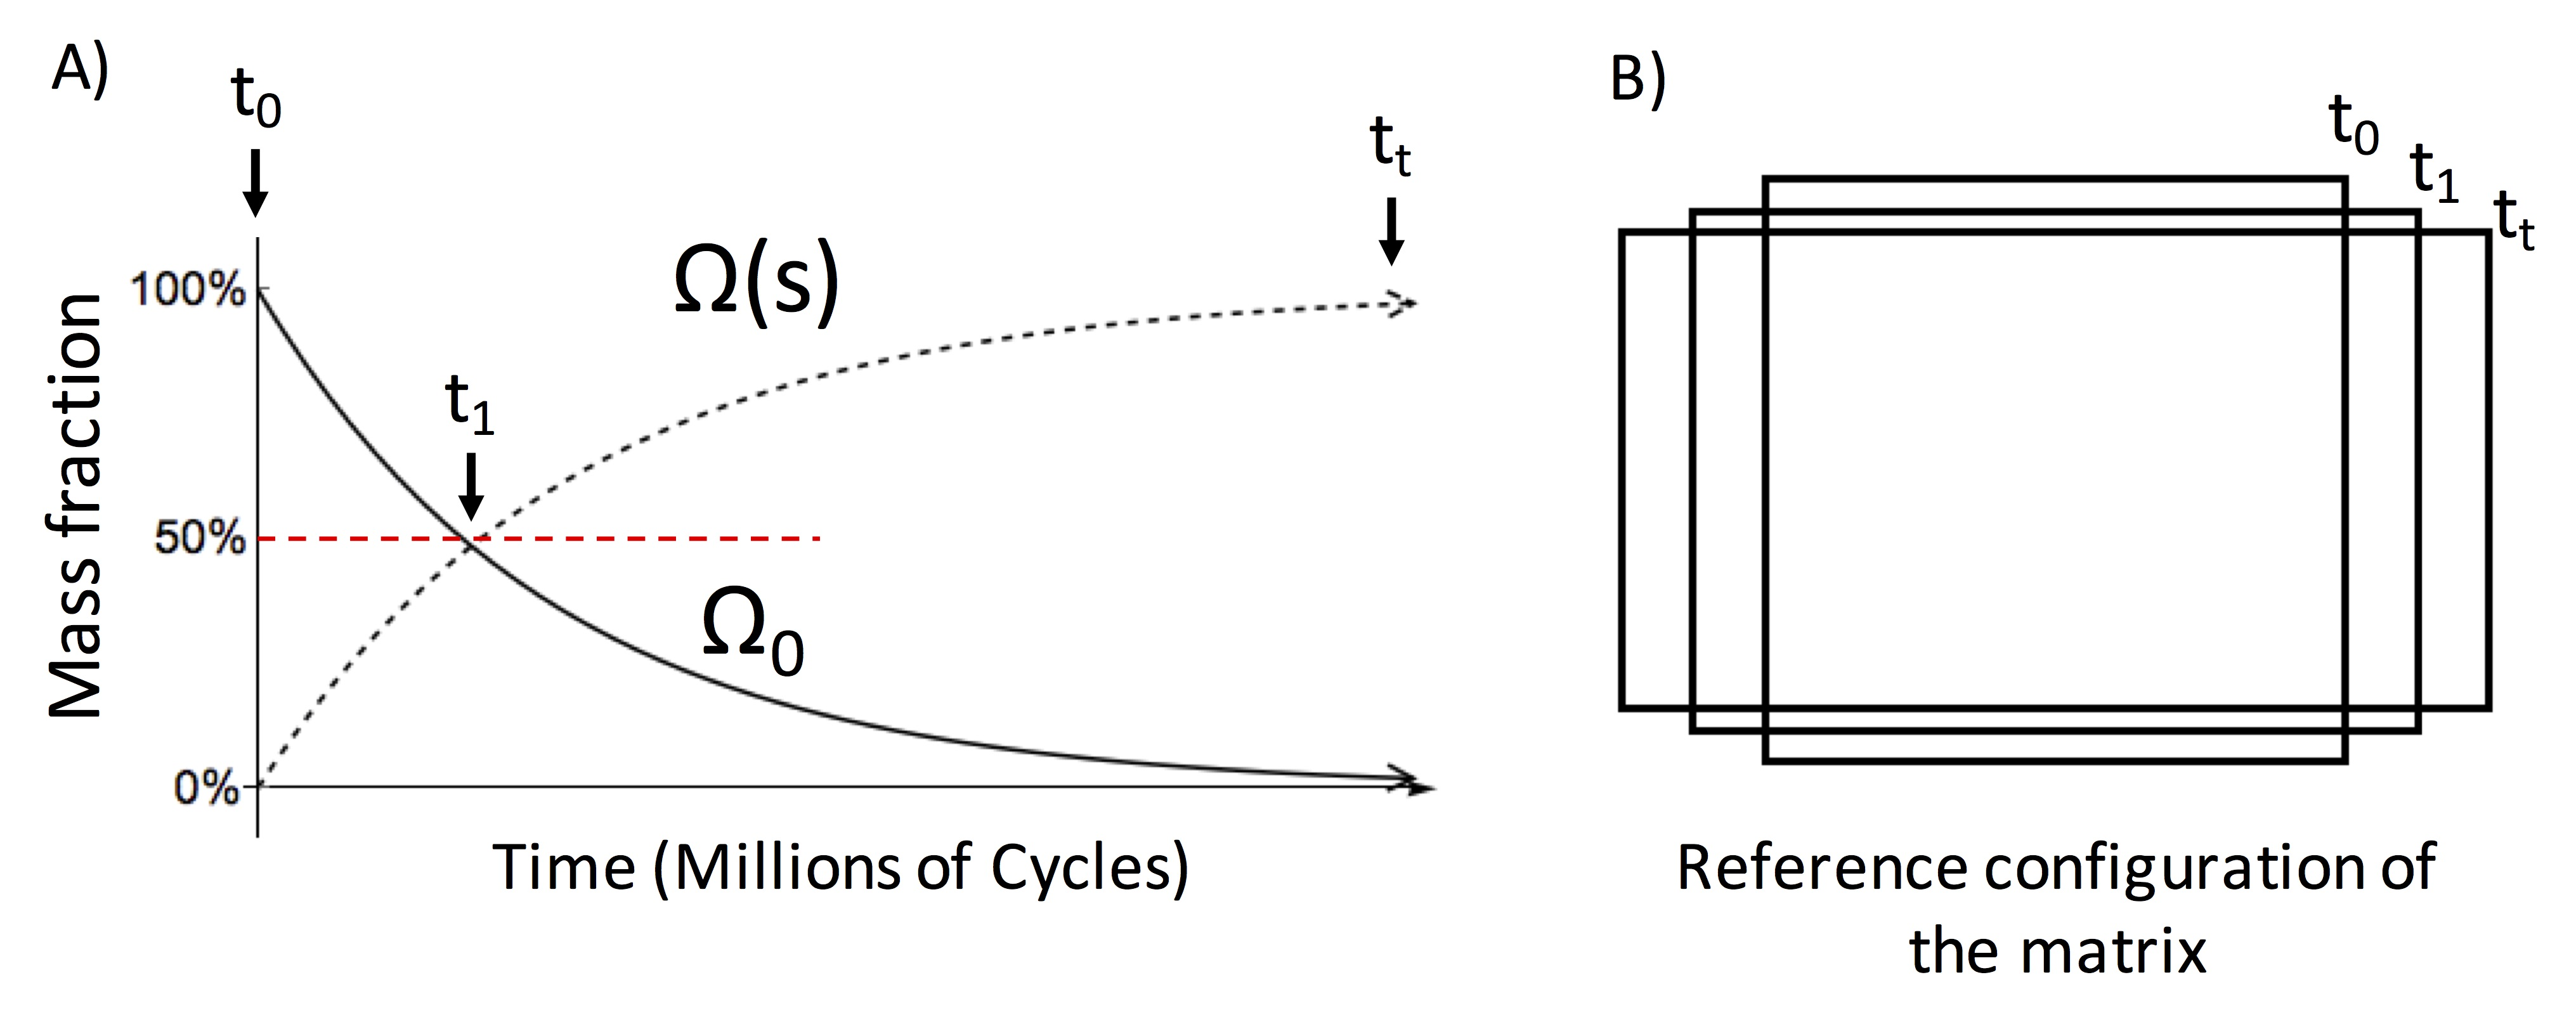
\includegraphics[width=\textwidth]{Images/chapter4/figure3}
\caption{Illustration of the permanent set effect under cyclic uniaxial loading. A) There is a transfer of mass fraction of the EXL matrix to the loaded configuration $\Omega(s)$ from the original state $\Omega_0$. B) This results in changes in the unloaded geometry of the tissue.}
\label{fig:PS}
\end{figure}

\begin{figure}[hbt]
\centering
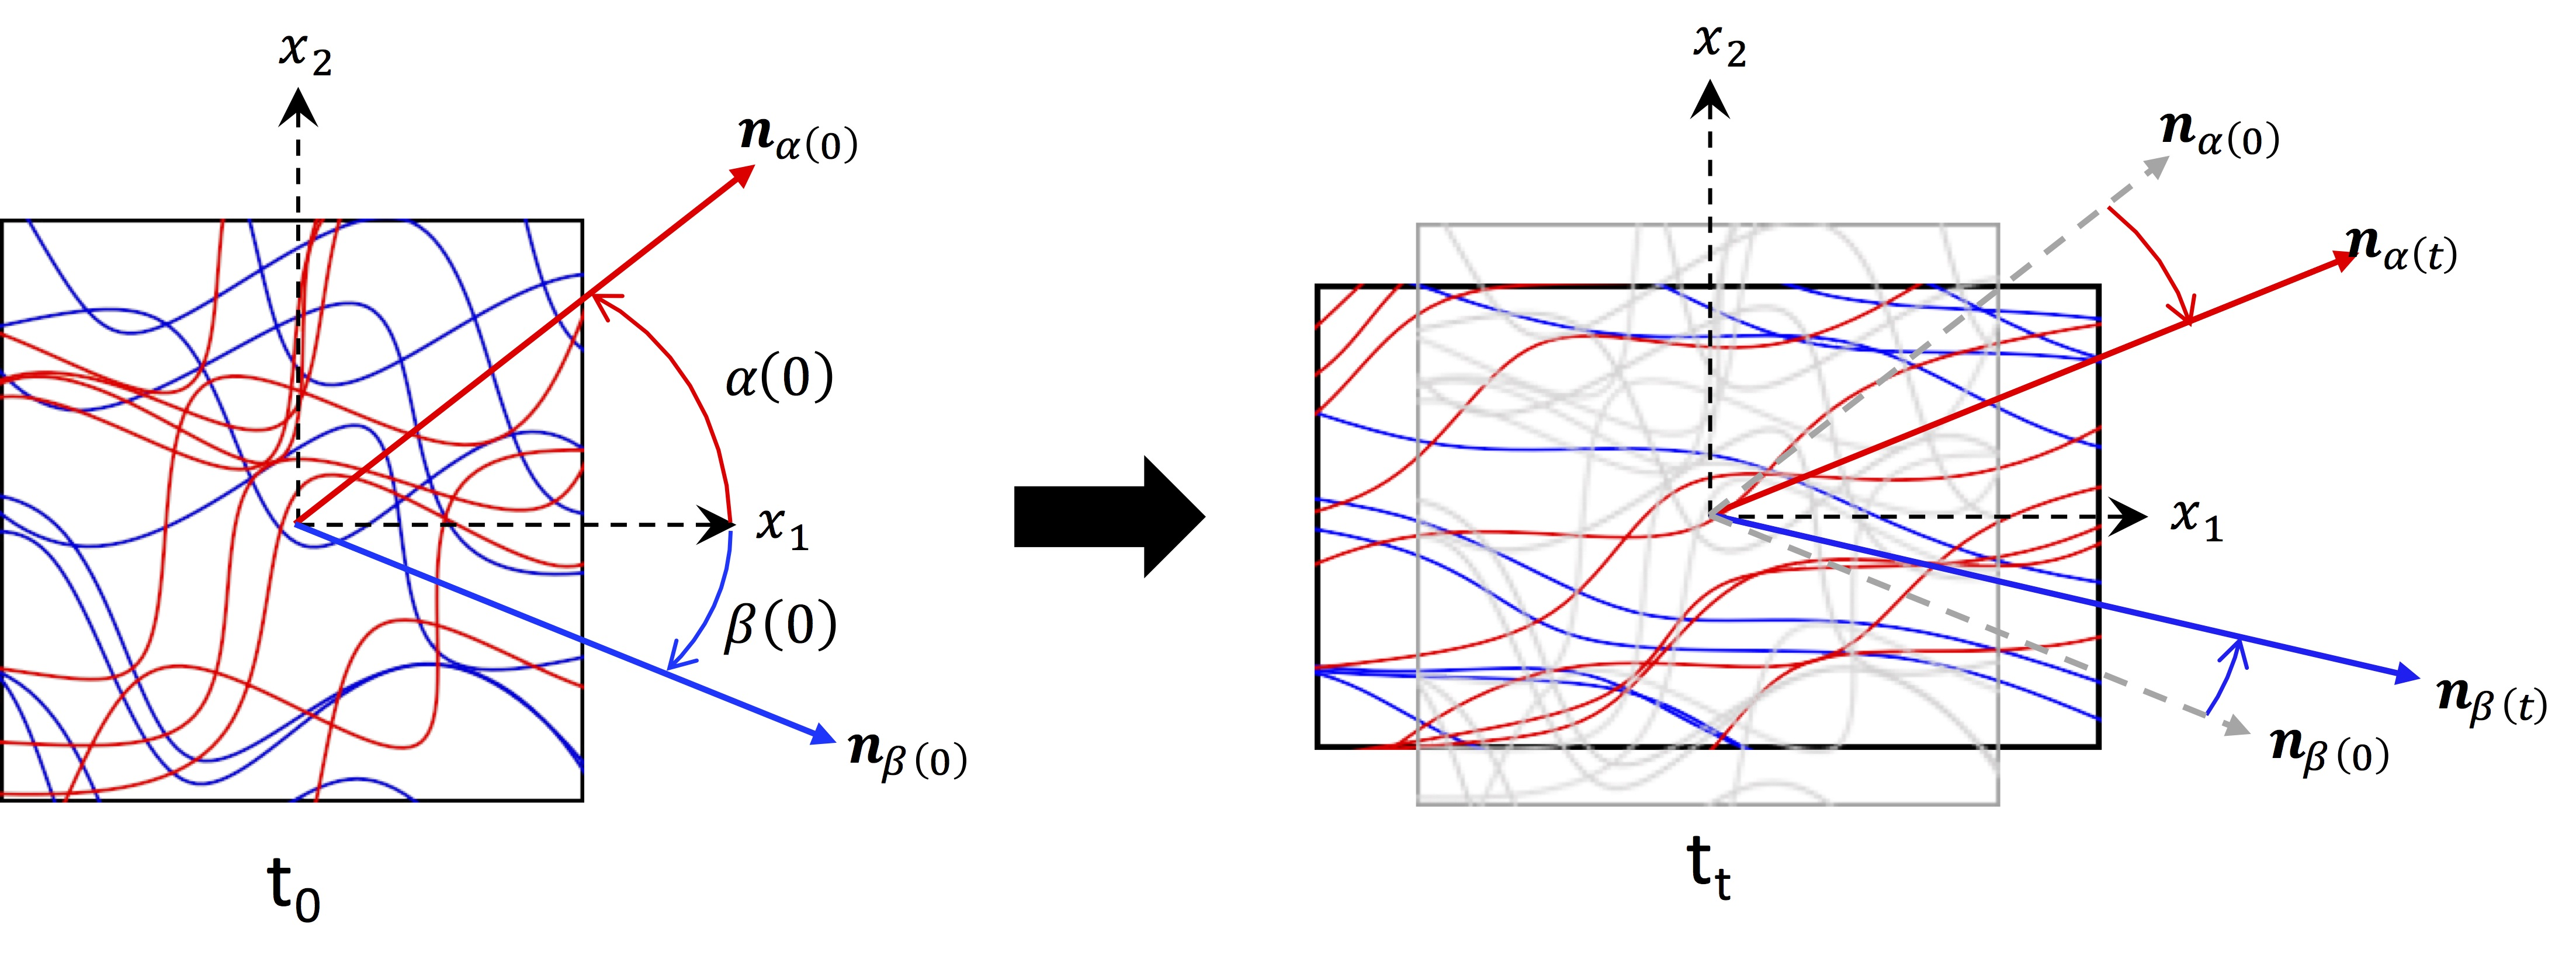
\includegraphics[width=\textwidth]{Images/chapter4/figure4}
\caption{An illustration of how the collagen fiber architecture is convected by changes in the dimension of the bulk tissue. The left figure shows the origin geometry of the tissue at $\mathrm{t}_0$ in figure \ref{fig:PS} while the right figure shows the geometry of the tissue at $\mathrm{t}_t$. Structural convection includes the rotation and straightening of the collagen fiber ensembles. }
\label{fig:structuralconvection}
\end{figure}


	To develop the constitutive model form, we start by modeling the exogenously crosslinked tissue under cyclic loading as parts of a mixture of materials with the same properties but different evolving reference states. The reference state of each part of the EXL matrix is updated according the strain history (Fig. \ref{fig:PS}A). The response of each part are then summed together for the bulk-level mechanical response of the EXL matrix. The new bulk level mechanical response is then used to determine the new unloaded state (Fig. \ref{fig:PS}B). The change in the EXL matrix from its uncycled state is then used to convect the collagen fiber architecture(Fig. \ref{fig:structuralconvection}). The new mechanical response of the EXL matrix is summed with the fiber ensemble interactions and collagen fiber response predicted from the new collagen fiber architecture to determine the full tissue-level mechanical response. Thus, how the \emph{collagen fiber architecture (CFA) is convected by the EXL matrix} is crucial to our model. We start developing our constitutive model by 1) modeling and parameter estimation for the native uncycled mechanical response of the exogenously crosslinked tissue. Then 2) develop the model form for the time evolving mechanical response based on the permanent set mechanism and cyclic loading data. The basic assumptions of our models are:
\begin{enumerate}
\item There is no structural damage to the collagen fibers or the EXL matrix
\item The crosslinking process that induce permanent set follows first order kinetics
\item We are only modeling permanent set under physiological conditions and the process is thus isothermal
\item Permanent set occurs in the isotropic EXL matrix, so that its rate constant is directionally independent
\item The permanent set rate constant is strain-level independent in the physiological range
\item Permanent set occurs over a time scale much longer than a single cardiac cycle
\item The tissue is functionally elastic, and thus viscoelastic effects are ignored
\item The convection of the collagen fiber architecture follows affine kinematics
\item collagen fibers do not bare load or interact until they are straightened
\cite{lee_presence_2015}
\end{enumerate}

